\documentclass{article}

\usepackage[LGR, T1]{fontenc}
\usepackage[utf8]{inputenc}
\usepackage[greek]{babel}
\usepackage{setspace}
\usepackage{amsmath}
\usepackage{graphicx}
\usepackage{caption}
\usepackage{subfiles}
\usepackage{graphicx}
\usepackage{subfig}
\graphicspath{ {./data/} }


\title{1η Εργασία Στο Μάθημα Της Αριθμητικής Ανάλυσης}
\doublespacing
\author{ Ονοματεπώνυμο : Παπαδόπουλος Αναστάσιος \\
            ΑΕΜ : 3654 \\
            Διδάσκων : Τέφας Αναστάσιος }

\begin{document}
\normalsize
\maketitle
\vspace{15px}
\begin{center}
    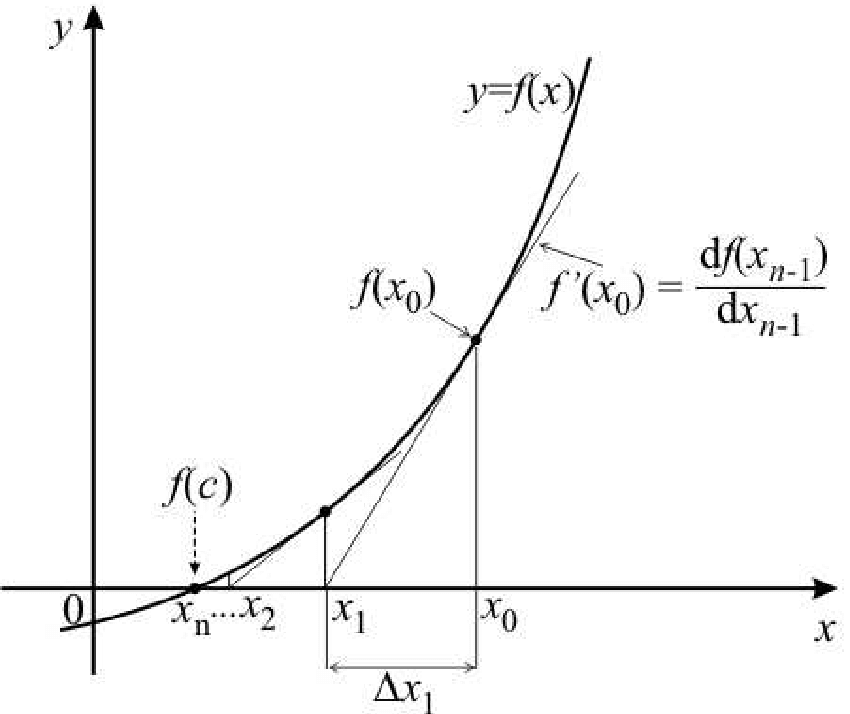
\includegraphics[scale=0.25]{intro_page_logo.png}
\end{center}
\begin{figure}[b]
    \begin{center}
        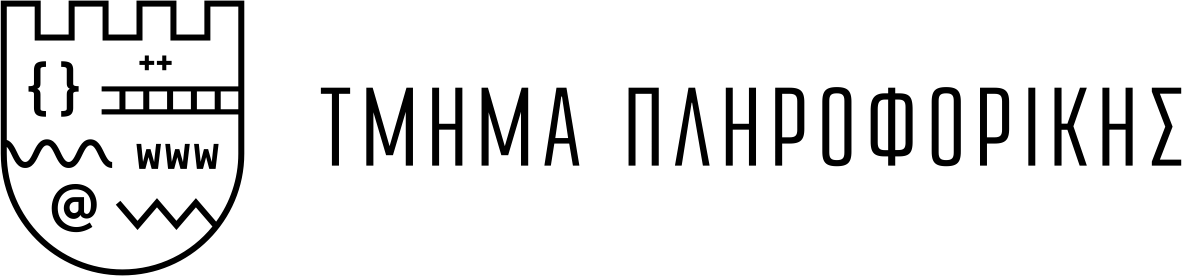
\includegraphics[scale=0.15]{csd_logo.png}    
    \end{center}
\end{figure}
\newpage
\doublespacing
\tableofcontents
\newpage

% Intro page
\subfile{intro.tex}

% Exercise 1 
\subfile{./Exercise1/exercise1.tex}
\subfile{./Exercise1/bisection.tex}
\subfile{./Exercise1/newton_raphson.tex}
\subfile{./Exercise1/secant.tex}
\subfile{./Exercise1/newton_converge.tex}
\subfile{./Exercise1/iterations_comparison.tex}

% Exercise 2
\subfile{./Exercise2/exercise2.tex}
\subfile{./Exercise2/modified_newton_raphson.tex}
\subfile{./Exercise2/modified_bisection.tex}
\subfile{./Exercise2/modified_secant.tex}
\subfile{./Exercise2/modified_bisection_converge.tex}
\subfile{./Exercise2/modified_vs_classic.tex}

% Exercise 3
\subfile{./Exercise3/exercise3.tex}
\subfile{./Exercise3/pa_lu_decomposition.tex}
\subfile{./Exercise3/cholesky_decomposition.tex}
\subfile{./Exercise3/gauss_seidel.tex}

% Exercise 4
\subfile{./Exercise4/exercise4.tex}
\subfile{./Exercise4/stohastic.tex}
\subfile{./Exercise4/dominant_eigenvector.tex}
\subfile{./Exercise4/improve_page_rank.tex}

\end{document}